\documentclass{ctexart}
\usepackage{tikz}
\begin{document}
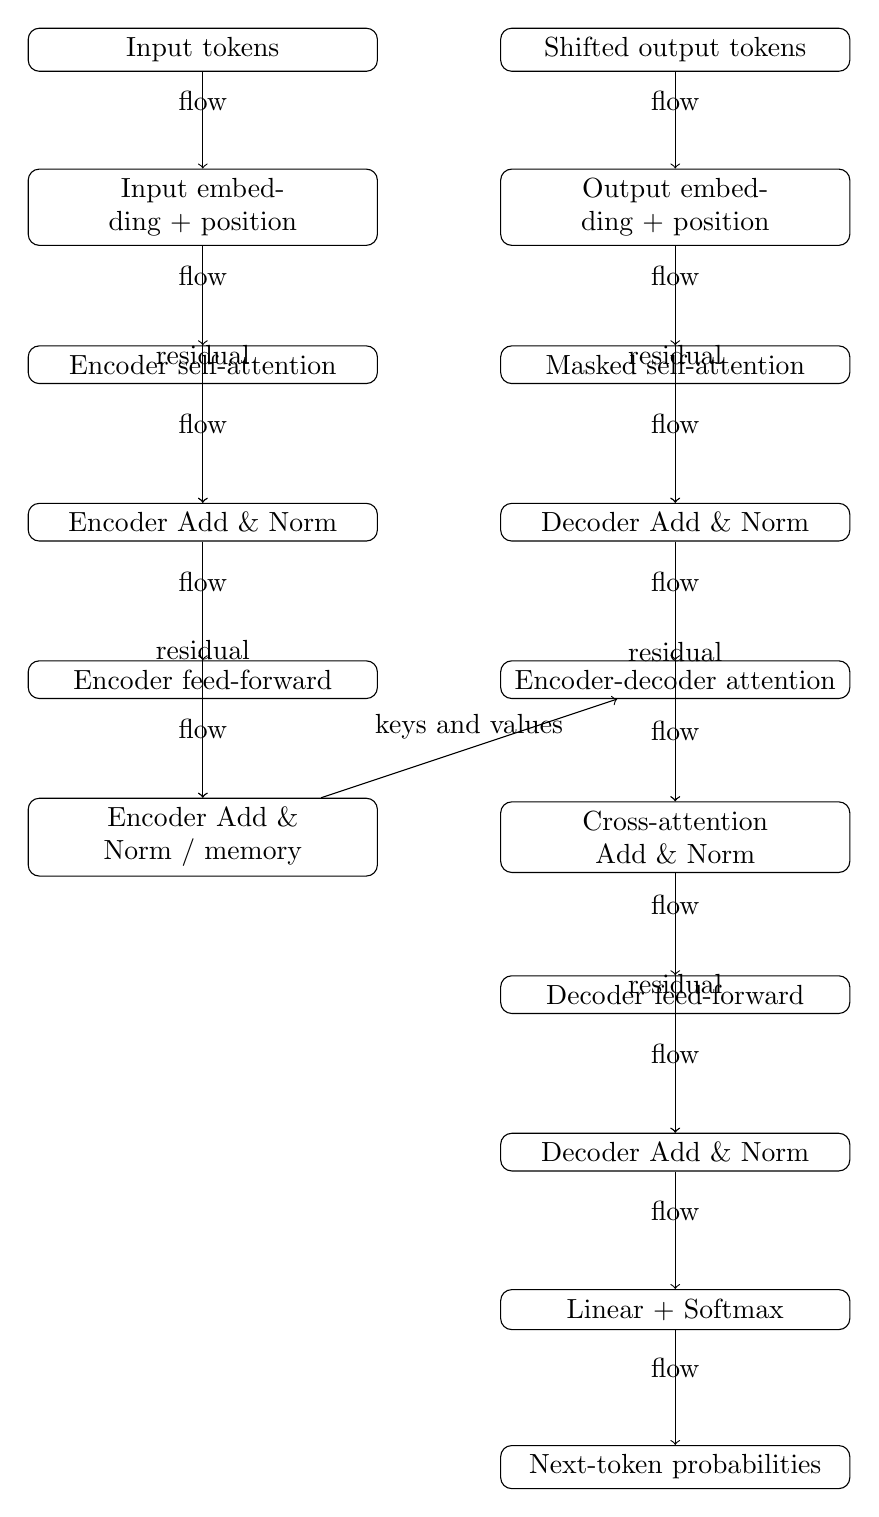
\begin{tikzpicture}[every node/.style={draw,rounded corners,align=center,text width=42mm}]
\node (n0) at (0,0) {Input tokens};
\node (n1) at (0,-2) {Input embedding + position};
\node (n2) at (0,-4) {Encoder self-attention};
\node (n3) at (0,-6) {Encoder Add \& Norm};
\node (n4) at (0,-8) {Encoder feed-forward};
\node (n5) at (0,-10) {Encoder Add \& Norm / memory};
\node (n6) at (6,0) {Shifted output tokens};
\node (n7) at (6,-2) {Output embedding + position};
\node (n8) at (6,-4) {Masked self-attention};
\node (n9) at (6,-6) {Decoder Add \& Norm};
\node (n10) at (6,-8) {Encoder-decoder attention};
\node (n11) at (6,-10) {Cross-attention Add \& Norm};
\node (n12) at (6,-12) {Decoder feed-forward};
\node (n13) at (6,-14) {Decoder Add \& Norm};
\node (n14) at (6,-16) {Linear + Softmax};
\node (n15) at (6,-18) {Next-token probabilities};
\draw[->] (n0) -- node[above,draw=none] {flow} (n1);
\draw[->] (n1) -- node[above,draw=none] {flow} (n2);
\draw[->] (n2) -- node[above,draw=none] {flow} (n3);
\draw[->] (n3) -- node[above,draw=none] {flow} (n4);
\draw[->] (n4) -- node[above,draw=none] {flow} (n5);
\draw[->] (n6) -- node[above,draw=none] {flow} (n7);
\draw[->] (n7) -- node[above,draw=none] {flow} (n8);
\draw[->] (n8) -- node[above,draw=none] {flow} (n9);
\draw[->] (n9) -- node[above,draw=none] {flow} (n10);
\draw[->] (n10) -- node[above,draw=none] {flow} (n11);
\draw[->] (n11) -- node[above,draw=none] {flow} (n12);
\draw[->] (n12) -- node[above,draw=none] {flow} (n13);
\draw[->] (n13) -- node[above,draw=none] {flow} (n14);
\draw[->] (n14) -- node[above,draw=none] {flow} (n15);
\draw[->] (n5) -- node[above,draw=none] {keys and values} (n10);
\draw[->] (n1) -- node[above,draw=none] {residual} (n3);
\draw[->] (n3) -- node[above,draw=none] {residual} (n5);
\draw[->] (n7) -- node[above,draw=none] {residual} (n9);
\draw[->] (n9) -- node[above,draw=none] {residual} (n11);
\draw[->] (n11) -- node[above,draw=none] {residual} (n13);
\end{tikzpicture}
\end{document}
